\chapter{Anhang}

\section{Verwendete Hilfsmittel}
In der Tabelle \ref{tab:tooling} sind die im Rahmen der Bearbeitung des Themas der \IthesisKindDE~verwendeten Werkzeuge und Hilfsmittel aufgelistet.

\begin{table}[!ht]
    \renewcommand{\arraystretch}{1.3}
    \begin{tabular}{|p{3cm}|p{10.5cm}|}
        \hline 
        \rowcolor{lightgray} \textbf{Tool} & \textbf{Verwendung} \\
        \hline
        \LaTeX & Textsatz- und Layout-Werkzeug zur Erstellung des Dokuments \\
        \hline
        ChatGPT & KI-gestützter Assistent zur Textgenerierung, Überarbeitung und Ideenfindung \\
        \hline
        ScholarGPT & Spezialisierte KI-Version zur Analyse wissenschaftlicher Quellen \\
        \hline
        Gemini & KI-Tool zur Unterstützung bei Recherche und Programmierung \\
        \hline
        Draw.io & Tool zur Erstellung von Diagrammen und technischen Skizzen \\
        \hline
        Google Colab & Cloudbasierte Python-Umgebung für Datenanalyse und Modellierung \\
        \hline
        Visual Studio Code & Quellcode-Editor zur Entwicklung und Bearbeitung von Programmdateien \\
        \hline
        Git & Versionskontrollsystem zur Nachverfolgung von Änderungen im Quellcode \\
        \hline
        Manifest v3 & Technische Spezifikation für die Erstellung von Chrome-Erweiterungen \\
        \hline
        HTML / CSS / JavaScript & Webtechnologien zur Umsetzung der Benutzeroberfläche \\
        \hline
    \end{tabular}
    \caption{Verwendete Hilfsmittel und Werkzeuge}
    \label{tab:tooling}
\end{table}

\newpage

In Tabelle \ref{tab:libs} folgen die verwendeten Bibliotheken und Frameworks.

\begin{table}[!ht]
    \renewcommand{\arraystretch}{1.3}
    \begin{tabular}{|p{3cm}|p{10.5cm}|}
        \hline 
        \rowcolor{lightgray} \textbf{Bibliothek / Framework} & \textbf{Verwendung} \\
        \hline
        Python & Programmiersprache zur Analyse, Automatisierung und Modellierung \\
        \hline
        pandas & Datenmanipulation und -analyse in Tabellenform \\
        \hline
        matplotlib & Erstellung von Diagrammen und Visualisierungen \\
        \hline
        numpy & Unterstützung für numerische Operationen und Arrays \\
        \hline
        scikit-learn & Implementierung klassischer ML-Algorithmen (z.B. Klassifikation) \\
        \hline
        transformers & Zugriff auf vortrainierte Sprachmodelle (z.B. BERT, GPT) \\
        \hline
        torch & Deep-Learning-Framework zur Implementierung neuronaler Netze \\
        \hline
        Hugging Face & Plattform und Bibliothek zur Bereitstellung von NLP-Modellen \\
        \hline
    \end{tabular}
    \caption{Verwendete Bibliotheken und Frameworks}
    \label{tab:libs}
\end{table}

\newpage

\section{Deklaration zur Nutzung von KI-gestützten Tools}

In dieser wissenschaftlichen Arbeit wurden Künstliche-Intelligenz (KI-Technologien) zur Unterstützung verschiedener Aspekte der Forschung eingesetzt. 
Die Nutzung umfasste unter anderem die Analyse und Auswertung von Literatur, die Unterstützung bei der Datenauswertung sowie die Generierung von Ideen und Inhalten.

Es wird ausdrücklich darauf hingewiesen, dass die endgültige Verantwortung für die inhaltliche Richtigkeit, die kritische Reflexion und die Interpretation der 
Ergebnisse beim Autor dieser Arbeit liegt.

Die KI diente lediglich als Werkzeug und nicht als Ersatz für das kritische und analytische Denken des Forschenden.

Tabelle \ref{tab:ki_nutzung} zeigt eine explizite Auflistung an welchen Stellen KI-Technologien verwendet wurden.

\begin{table}[!ht]
    \centering
    \begin{tabular}{|p{3cm}|p{10.5cm}|}
        \hline
        \rowcolor{lightgray} \textbf{Abschnitt / Kapitel} & \textbf{Art der Unterstützung durch KI} \\
        \hline
        Kapitel \ref{chap:einleitung} & 
            \begin{itemize}[leftmargin=*,noitemsep,topsep=0pt,partopsep=0pt]
                \item Ideenfindung zum Aufbau des Kapitels
                \item Zusammenfassen wissenschaftlicher Arbeiten, Definitionen und Nachrichtenartikeln
                \item Formulierung von Einleitungen
            \end{itemize} \\
        \hline
        Kapitel \ref{chap:nlp} & 
            \begin{itemize}[leftmargin=*,noitemsep,topsep=0pt,partopsep=0pt]
                \item Formulierung von Einleitungen
                \item Zusammenfassen wissenschaftlicher Arbeiten
                \item Ausformulierung von Stichpunkten
                \item Unterstützung bei der sprachlichen Glättung und Terminologieerklärung zu den verschiedenen Modellen
                \item Erstellung von Tabelle \ref{tab:vergleich} und Tabelle \ref{tab:linkfunktionen}
                \item Schrittweise Erklärung der Funktionalität von LightGBM, Self-Attention und Hidden-Layer
                \item Beispiel WordPiece Embedding und BPE
                \item Self-Attention Beispiel in Kapitel \ref{sec:self_attention}
                \item Übersetzung der Dokumentation von RoBERTa in Kapitel \ref{sec04:roberta}
            \end{itemize} \\
        \hline
        Kapitel \ref{chap:relevante_datensaetze_und_auswahlkriterien} & 
            \begin{itemize}[leftmargin=*,noitemsep,topsep=0pt,partopsep=0pt]
                \item RKI-Satz Beispiel in Kapitel \ref{sec:english_datasets}
            \end{itemize} \\
        \hline
        Kapitel \ref{chap:konzeption_der_softwareloesung} & 
            \begin{itemize}[leftmargin=*,noitemsep,topsep=0pt,partopsep=0pt]
                \item Erstellung von Tabelle \ref{table:technischeAnsaetze}
                \item Formulierung von Einleitungen und Beschreibungen
            \end{itemize} \\
        \hline
        Kapitel \ref{chap:umsetzung_des_prototyps} &
            \begin{itemize}[leftmargin=*,noitemsep,topsep=0pt,partopsep=0pt]
                \item Schrittweise Erklärung des Codes in Kapitel \ref{sec:erzeugung_der_embeddings}
                \item Erstellung der UML Klasse (Abbildung \ref{fig:uml_webserver})
                \item Formulierung von Einleitungen
            \end{itemize} \\
        \hline
        Kapitel \ref{chap:evaluation_und_ergebnisse} & 
            \begin{itemize}[leftmargin=*,noitemsep,topsep=0pt,partopsep=0pt]
                \item Erstellung der Latex Tabellen anhand von Logging Daten und Outputs
                \item Teilweise Erstellungen von schriftlichen Beschreibungen und Vergleichen der Tabellen
            \end{itemize} \\
        \hline
        Kapitel \ref{chap:fazit} \& Kapitel \ref{chap:ausblick} & Ausformulieren von gesammelten Stichpunkten \\
        \hline
    \end{tabular}
    \caption{Dokumentation der Nutzung KI-gestützter Hilfsmittel}
    \label{tab:ki_nutzung}
\end{table}

\newpage

\section{Abbildungen}

\begin{figure}[htbp]
    \begin{center}
        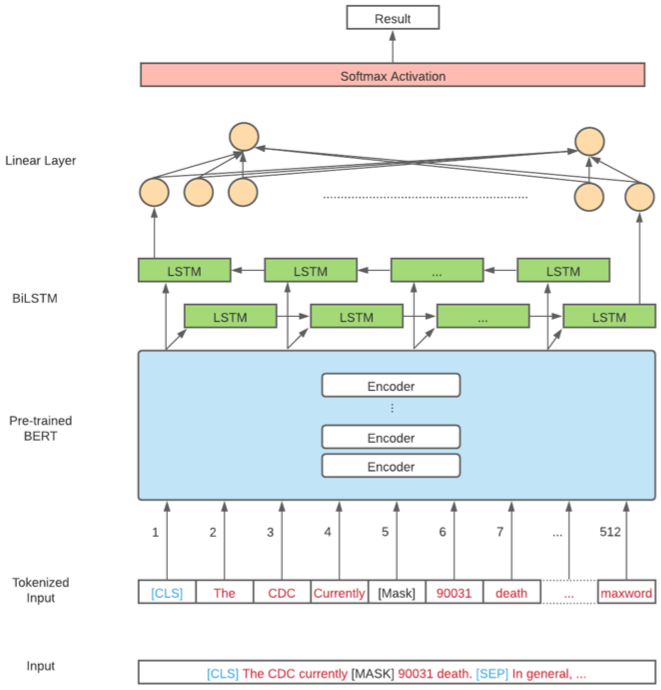
\includegraphics[scale=0.6]{static/bert_bilstm_architecture.png}
        \caption{\label{fig:bert_bilstm_architecture} Architektur des hybriden Modells \cite{wang2021covid19fakenewsdetection}}
    \end{center}
\end{figure}

\begin{figure}[htbp]
    \begin{center}
        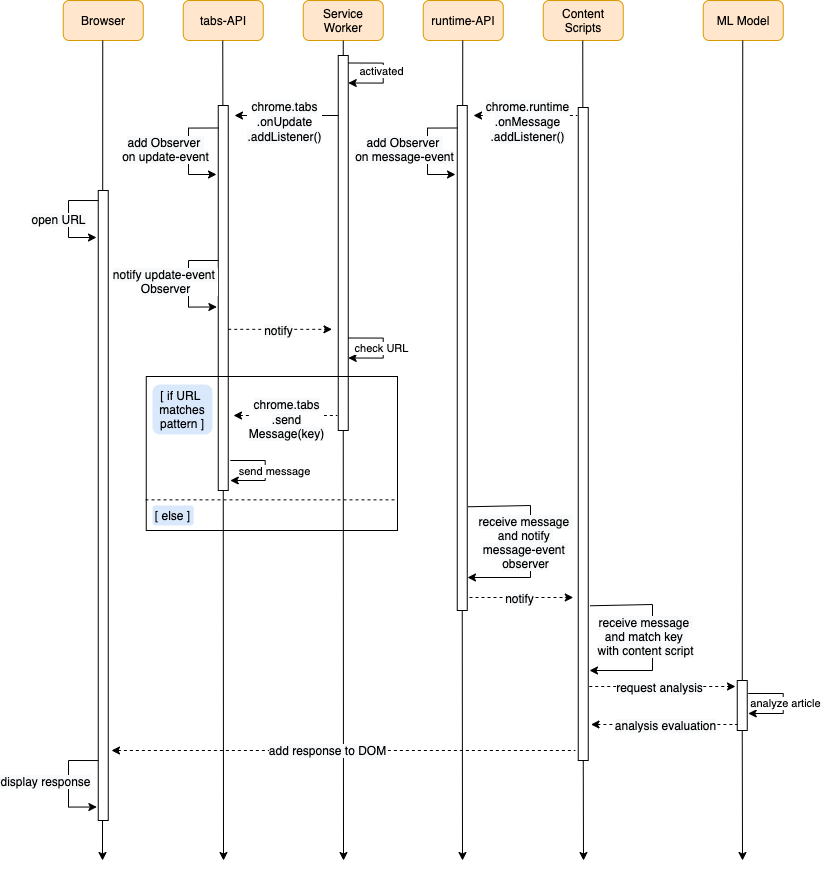
\includegraphics[width=\linewidth]{diagrams/hauptkomponente_sequenzdiagramm.png}
        \caption{\label{fig:seq_hauptkomponente} Sequenzdiagramm Webagent}
    \end{center}
\end{figure}

\begin{figure}[htbp]
    \begin{center}
        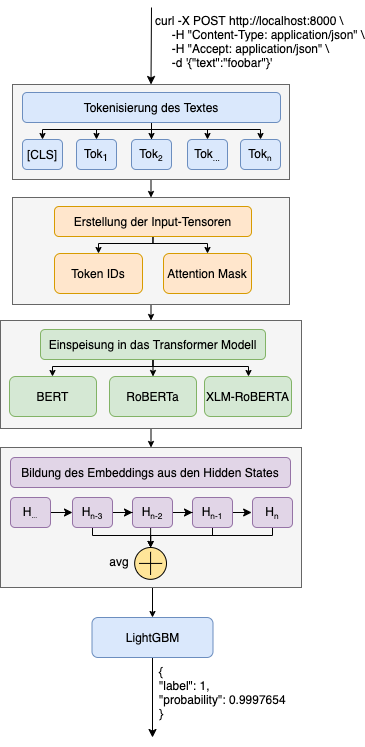
\includegraphics[scale=0.6]{diagrams/gesamtarchitektur.png}
        \caption{\label{fig:gesamtarchitektur} Gesamtarchitektur des Webservers}
    \end{center}
\end{figure}

\newpage

\section{Tabellen}

\begin{table}[htbp]
    \centering
    \renewcommand{\arraystretch}{1.3}
    \begin{tabular}{|p{2.5cm}|p{2.5cm}|p{2.5cm}|p{2.5cm}|p{2.5cm}|}
        \hline
        \rowcolor{lightgray} \textbf{Kriterium} & \textbf{Chrome Extension} & \textbf{Userscript (Tampermonkey)} & \textbf{Proxy-Server} & \textbf{Scraper + Plattform} \\
        \hline
        DOM-Zugriff beim Nutzer & Ja & Ja & Nein & Nein \\
        \hline
        Einbindung auf \texttt{bild.de} direkt & Ja & Ja & Ja (indirekt) & Nein \\
        \hline
        Installation durch Nutzer & Mittel & Einfach & Nicht erforderlich & Nicht erforderlich\\
        \hline
        Komplexität der Umsetzung & Mittel & Gering & Hoch & Mittel \\
        \hline
        Wartbarkeit \& Updates & Gut & Gut & Aufwändig & Mittel \\
        \hline
        Performance beim Nutzer & Hoch & Hoch & Hoch & Hoch \\
        \hline
        Skalierbarkeit & Hoch & Eingeschränkt & Mittel & Hoch \\
        \hline
        Für öffentliche Verbreitung geeignet & Ja & Eingeschränkt & Eingeschränkt & Ja \\
        \hline
        API-Nutzung zur Fake-Erkennung & Ja & Ja & Ja & Ja \\
        \hline
        Entwickler-kontrolle über UI & Hoch & Mittel & Hoch & Mittel \\
        \hline
    \end{tabular}
    \caption{Vergleich möglicher Technologien für den Webagenten}
    \label{table:technischeAnsaetze}
\end{table}


\begin{sidewaystable}[htbp]
    \centering
    \renewcommand{\arraystretch}{1.3}
    \begin{tabular}{|p{3.5cm}|p{2.8cm}|p{2.8cm}|p{2.8cm}|p{2.8cm}|p{2.8cm}|}
        \hline
        \rowcolor{lightgray} \textbf{Merkmal} & \textbf{BERT Base} & \textbf{RoBERTa\newline Base} & \textbf{RoBERTa Large} & \textbf{XLM-RoBERTa Base} & \textbf{XLM-RoBERTa Large} \\
        \hline
        \textbf{Hidden Size} & 768 & 768 & 1024 & 768 & 1024 \\
        \hline
        \textbf{Anzahl Layer} & 12 & 12 & 24 & 12 & 24 \\
        \hline
        \textbf{Anzahl Attention Heads} & 12 & 12 & 16 & 12 & 16 \\
        \hline
        \textbf{Vocab Size} & 30,522 & 50,265 & 50,265 & 250,002 & 250,002 \\
        \hline
        \textbf{Spezialisiert auf} & Masked LM & Masked LM & Masked LM & Multilinguales Masked LM & Multilinguales Masked LM \\
        \hline
        \textbf{Sprachumfang} & Englisch & Englisch & Englisch & Multilingual & Multilingual \\
        \hline
    \end{tabular}
\caption{Vergleich der verschiedenen BERT- und RoBERTa-Modelle}
\label{tab:bert_models}
\end{sidewaystable}

\begin{table}[htbp]
    \centering
    \renewcommand{\arraystretch}{1.3}
    \begin{tabular}{|p{3cm}|l|p{6cm}|}
        \hline
        \rowcolor{lightgray} \textbf{Parameter} & \textbf{Wert} & \textbf{Beschreibung} \\
        \hline
        Anzahl Trainingsepochen & \texttt{5} & Das gesamte Trainingsset wird fünfmal vollständig durchlaufen. \\
        \hline
        Batch-Größe & \texttt{32} & Anzahl der Beispiele, die gleichzeitig in einem Schritt verarbeitet werden. \\
        \hline
        Lernrate & \texttt{2e-5} & Bestimmt die Schrittweite der Modellaktualisierung bei jedem Optimierungsschritt. \\
        \hline
        Optimierungs-verfahren & \texttt{AdamW} & Variante des Adam-Optimierers mit Weight Decay, automatisch in Hugging Face integriert. \\
        \hline
        Gewichtsabnahme (Weight Decay) & \texttt{0.01} & Reguliert große Gewichtswerte, um Überanpassung zu vermeiden. \\
        \hline
        Lernraten-Scheduler & \texttt{Linear, 10\% Warmup} & Die Lernrate steigt linear an und wird anschließend schrittweise reduziert. \\
        \hline
        Kriterium für bestes Modell & \texttt{F1-Score} & Das Modell mit dem besten F1-Score auf den Validierungsdaten wird gespeichert. \\
        \hline
        Hardware-Beschleunigung & \texttt{fp16 aktiviert} & Angepasst auf A100 GPU zur Beschleunigung des Trainings. \\
        \hline
    \end{tabular}
    \caption{Überblick über die gewählten Hyperparameter der Transformer-Modelle}
    \label{tab:transformer-hyperparameter}
\end{table}


\begin{table}[htbp]
    \centering
    \renewcommand{\arraystretch}{1.1}
    \begin{tabular}{|p{3cm}|l|p{7cm}|}
        \hline
        \rowcolor{lightgray} \textbf{Parameter} & \textbf{Wert} & \textbf{Beschreibung} \\
        \hline
        Ziel (\texttt{objective}) & \texttt{binary} & Binäre Klassifikation (z.\,B. „echt“ oder „fake“). \\
        \hline
        Metrik (\texttt{metric}) & \texttt{binary\_logloss} & Verlustfunktion zur Bewertung der Modellgüte während des Trainings. \\
        \hline
        Boosting-Typ (\texttt{boosting\_type}) & \texttt{gbdt} & Verwendung von Gradient Boosted Decision Trees als Lernverfahren. \\
        \hline
        Prozessor-Kerne (\texttt{n\_jobs}) & \texttt{-1} & Nutzt alle verfügbaren CPU-Kerne für paralleles Training. \\
        \hline
        Lernrate (\texttt{learning\_rate}) & \texttt{0.0865} & Schrittweite beim Anpassen der Modellgewichte. \\
        \hline
        Anzahl Blätter (\texttt{num\_leaves}) & \texttt{63} & Maximale Anzahl von Blättern pro Entscheidungsbaum. \\
        \hline
        Maximale Tiefe (\texttt{max\_depth}) & \texttt{20} & Begrenzt die Tiefe der Bäume zur Kontrolle der Komplexität. \\
        \hline
        Min. Samples pro Blatt (\texttt{min\_child\_samples}) & \texttt{80} & Minimale Anzahl an Trainingsbeispielen pro Blatt. \\
        \hline
        Subsample-Rate (\texttt{subsample}) & \texttt{0.9818} & Anteil der Trainingsdaten, der zufällig pro Baum verwendet wird. \\
        \hline
        Merkmalsauswahl pro Baum (\texttt{colsample\_bytree}) & \texttt{0.9684} & Anteil der Merkmale, die pro Baum zufällig ausgewählt werden. \\
        \hline
        $L_1$-Regularisierung (\texttt{reg\_alpha}) & \texttt{0.2989} & Bestraft große Gewichtswerte zur Förderung einfacher Modelle. \\
        \hline
        $L_2$-Regularisierung (\texttt{reg\_lambda}) & \texttt{0.4609} & Stabilisiert das Modell durch Bestrafung großer Gewichtssummen. \\
        \hline
        Zufallsstart (\texttt{random\_state}) & \texttt{42} & Sichert Reproduzierbarkeit der Ergebnisse. \\
        \hline
        Anzahl Bäume (\texttt{n\_estimators}) & \texttt{2000} & Maximale Anzahl an Bäumen; Early Stopping begrenzt effektiv. \\
        \hline
    \end{tabular}
    \caption{Überblick über die gewählten Hyperparameter des LightGBM-Modells}
    \label{tab:lightgbm-hyperparameter}
\end{table}